\documentclass[11pt]{article}

\usepackage{amsmath, amssymb, amsthm}
\usepackage{tikz}

\theoremstyle{plain}
\newtheorem{thm}{Theorem}[section]
\newtheorem*{thm*}{Theorem}
\newtheorem{prop}[thm]{Proposition}
\newtheorem{lem}[thm]{Lemma}
\newtheorem*{lem*}{Lemma}
\newtheorem{dfn}[thm]{Definition}
\newtheorem{cor}[thm]{Corollary}
\newtheorem{claim}[thm]{Claim}
\newtheorem{conj}[thm]{Conjecture}
\newtheorem{ques}[thm]{Question}
\newtheorem*{rem}{Remark}


\oddsidemargin  0pt
\evensidemargin 0pt
\marginparwidth 40pt
\marginparsep 10pt
\topmargin 0pt
\headsep 10pt
\textheight 8.2in
\textwidth 6.4in
\renewcommand{\baselinestretch}{1.1}

\newcommand{\codeg}{\text{codeg}}
\newcommand{\BBE}{\mathbb{E}}
\newcommand{\BFP}{\mathbf{P}}
\usepackage{amsmath}
\usepackage{amsthm}
\usepackage{amssymb}
\usepackage{mathtools}
\usepackage{hyperref}
\usepackage{url}





\usepackage{graphicx}
\usepackage{caption}
\usepackage{subcaption}

\def\eQb#1\eQe{\begin{eqnarray*}#1\end{eqnarray*}}
\def\eQnb#1\eQne{\begin{eqnarray}#1\end{eqnarray}}
\providecommand{\e}[1]{\ensuremath{\times 10^{#1}}}
\providecommand{\pb}[0]{\pagebreak}
\DeclarePairedDelimiter\ceil{\lceil}{\rceil}
\DeclarePairedDelimiter\floor{\lfloor}{\rfloor}

\newcommand{\E}{\mathrm{E}}
\newcommand{\Var}{\mathrm{Var}}
\newcommand{\Cov}{\mathrm{Cov}}

\def\Qb#1\Qe{\begin{question}#1\end{question}}
\def\Sb#1\Se{\begin{solution}#1\end{solution}}


\newtheoremstyle{quest}{\topsep}{\topsep}{}{}{\bfseries}{}{ }{\thmname{#1}\thmnote{ #3}.}
\theoremstyle{quest}
\newtheorem*{definition}{Definition}
\newtheorem*{theorem}{Theorem}
\newtheorem*{lemma}{Lemma}
\newtheorem*{question}{Question}
\newtheorem*{preposition}{Preposition}
\newtheorem*{exercise}{Exercise}
\newtheorem*{challengeproblem}{Challenge Problem}
\newtheorem*{solution}{Solution}
\newtheorem*{remark}{Remark}
\usepackage{verbatimbox}
\usepackage{listings}
\usepackage{mathrsfs}
\date{}
\title{\vspace{-0.7cm}
Diff Geo II: Problem Set II}

\author{
Youngduck Choi 
\thanks{Department of Mathematics, Courant Institute of Mathematical Sciences, 
yc1104@nyu.edu; If you find an error and want to share with me, 
you can reach me via email.
}}

\begin{document}

\maketitle

\begin{abstract}
This work contains solutions for the problem set II.
\end{abstract}


\begin{question}[1-1]
\hfill
\begin{figure}[h!]
  \centering
    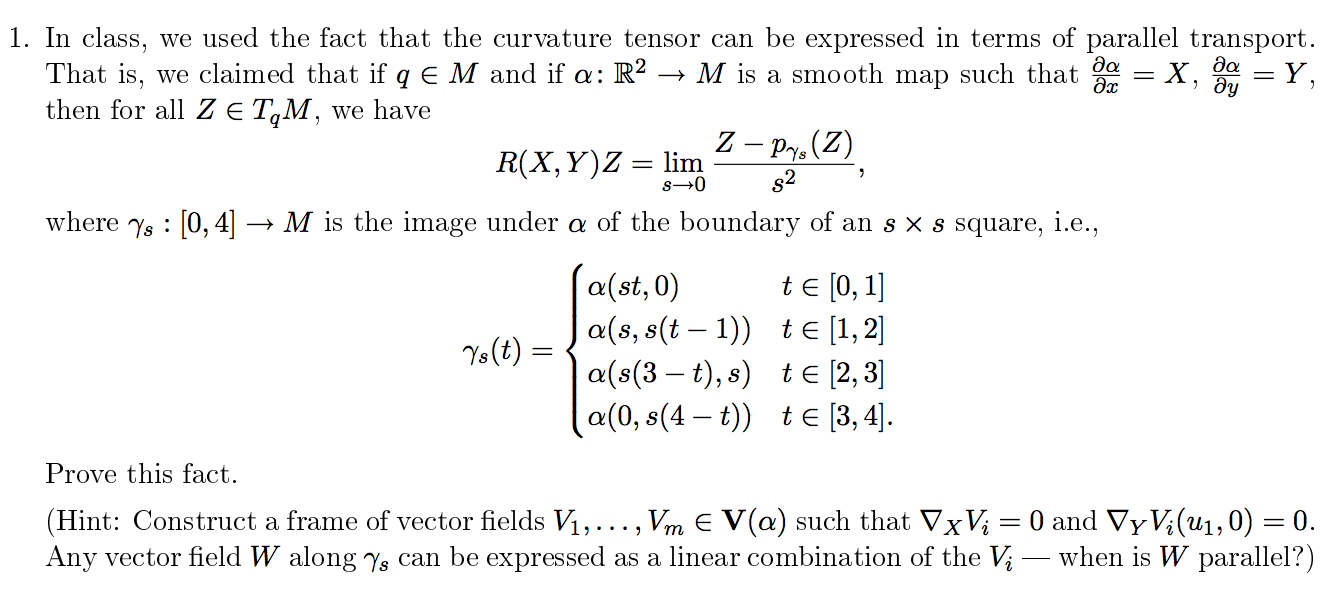
\includegraphics[width=0.7\textwidth]{geoII-s2-p1.png}
\end{figure}
\end{question}
\begin{solution} \hfill \\
Let $s > 0$. Set
\eQb
V_i(\alpha(s_1,s_2)) = P_{\alpha(0,s_2),\alpha(s_1,s_2)} \circ P_{q,\alpha(0,s_2)}(
V_i(q))
\eQe
for all $1 \leq i \leq m$ and $(s_1,s_2) \in [0,s]\times[0,s]$. As $\dfrac{\partial 
\alpha}{\partial x} = X$, $\dfrac{\partial \alpha}{\partial y} = Y$, we have
\eQb
\triangledown_{X} V_i = 0 \>\>\> &\text{and}& \>\>\>  \triangledown_Y V_i(u_1,0) = 0 
\eQe 
for all $i$. Then, we see that any $W \in V(\gamma)$ can only change along 2nd part 
of the path. We compute 
\eQb
V_i(q)(P_{\gamma}W(q)-W(q)) &=& <V_i,W>\gamma_s(2) + <V_i,W>\gamma_s(1) \\
&=& \int_{0}^{s} \partial_t <V_i,W>dt = \int_{0}^{s} V_i \cdot \triangledown_{Y}
W(1,t) dt \\
&=& \int_{0}^{s} V_i \cdot \triangledown_{Y}W(1,t) dt - \int_{0}^{s} \partial_r(
V_i \cdot \triangledown_{Y}W(r,t) drdt \\
&=& -\int_{0}^{s} \int_{0}^{s} V_i \cdot \triangledown_{X}\triangledown_{Y} W(r,t)
drdt  
\eQe
for all $i$. Now, with $W(0,0) = Z$, and $[X,Y] = 0$, letting $s \downarrow 0$, gives
\eQb
\lim_{s \downarrow 0} \dfrac{<Z-P_{\gamma}(Z), V_i>}{s^2} = <R(X,Y)Z,V_i>
\eQe
for all $i$, and hence,
\eQb
R(X,Y)Z = \lim_{s \downarrow 0} \dfrac{Z - P_{\gamma}(Z)}{s^2}.
\eQe
\hfill $\qed$

\end{solution}


\newpage

\begin{question}[1-2]
\hfill
\begin{figure}[h!]
  \centering
    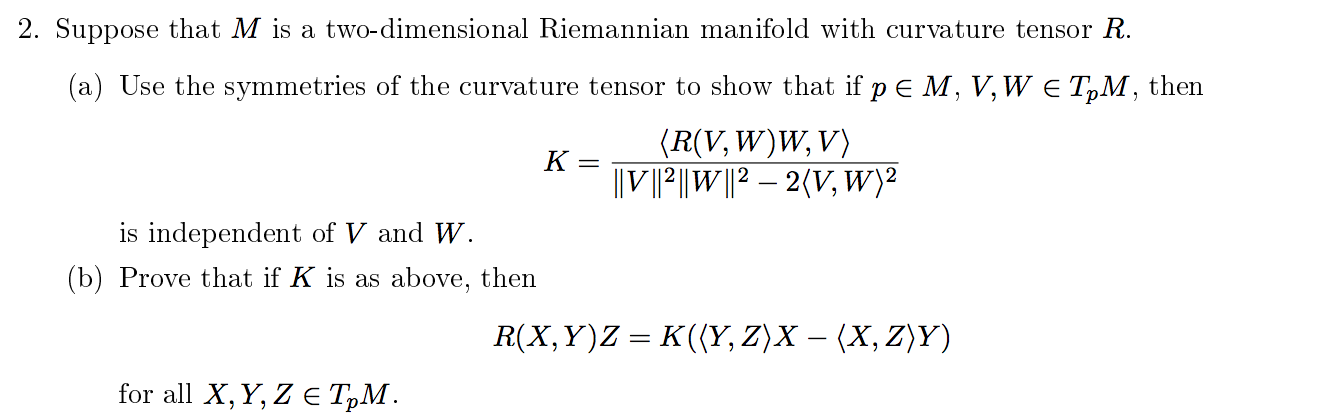
\includegraphics[width=0.7\textwidth]{geoII-s2-p2.png}
\end{figure}
\end{question}
\begin{solution} \hfill \\
I believe there is a typo in the problem: 2 in the denominator should be gone. 

\bigskip

\noindent 
\textbf{(a)}
Let $E_1, E_2$ be orthonormal frame, so $V = V^1 E_1 + V^2 E_2$ and $W = 
W^1 E_1 + W^2 E_2$. Then,
\eQnb
< R(V,W)W,V> &=& <R(V^1 E_1 + V^2 E_2 , W^1 E_1 + W^2 E_2)W,V> \nonumber \\
&=& <V^1W^2R(E_1,E_2)W,V> + <V^2W^1R(E_2,E_1)W,V> \label{eq:1-2-1} \\
&=& (V^1W^2 - V^2W^1)(W^1V^2<R(E_1,E_2)E_1,E_2> + W^2V^1<R(E_1,E_2)E_2,E_1>) 
\nonumber \\
&=& -(V^1W^2 - V^2W^1)^2 <R(E_1,E_2)E_1,E_2> \nonumber 
\eQne 
where~\eqref{eq:1-2-1}, in particular, holds by $R(E_1,E_1)W =R(E_2,E_2)W = 0$.
Furthermore,
\eQb
||V||^2||W||^2 - <V,W>^2 &=& (V^1W^2-V^2W^1)^2 \\
\eQe 
and hence
\eQb
K &=& \dfrac{-(V^1W^2 - V^2W^1)^2<R(E_1,E_2)E_1,E_2>}{(V^1W^2 - V^2W^1)^2} \\
&=& <R(E_1,E_2)E_2,E_1>
\eQe
Therefore, we see that $K$ only depend on the chosen frame, so $K$
is independent of $V$ and $W$.

\bigskip

\noindent \textbf{(b)} We compute
\eQb
R(X,Y)Z &=& \sum_{i,j,k = 1}^2 X^iY^jZ^k R(E_i,E_j) E_k \nonumber \\
&=& (X^1Y^2Z^1 - X^2Y^1Z^1) R(E_1,E_2) E_1 + (X^1Y^2Z^2 - X^2 Y^1Z^2) R(E_1,E_2)E_2 \\ 
\eQe
and
\eQb
K(<Y,Z>X - <X,Z>Y) &=& <R(E_1,E_2)E_2, E_1> X (Y^1Z^1 + Y^2 Z^2) \\ 
&-& <R(E_1,E_2)E_2,E_1> Y(X^1Z^1 + X^2 Z^2) \\
&=& <R(E_1,E_2)E_2,E_1>(X^1Y^2Z^2 - X^2Z^2Y^1)E_1 \\
&+& <R(E_1,E_2)E_2,E_1>(Y^1Z^1X^2 - X^1Y^2Z^1)E_2
\eQe
Therefore, 
\eQb
<R(X,Y)Z, E_1> &=& <R(E_1,E_2)E_2,E_1>(X^1Y^2Z^2 - X^2Y^1Z^2) \\
&=& <K(<Y,Z>X - <X,Z>Y),E_1> \\
\eQe
Similarly,
\eQb
<R(X,Y)Z, E_2> &=&  <K(<Y,Z>X - <X,Z>Y),E_2>.
\eQe
As the equality holds for the basis elements, we have
\eQb
R(X,Y)Z &=& K(<Y,Z>X - <X,Z>Y) 
\eQe
as required. \hfill $\qed$

\end{solution}

\newpage

\begin{question}[1-3]
\hfill
\begin{figure}[h!]
  \centering
    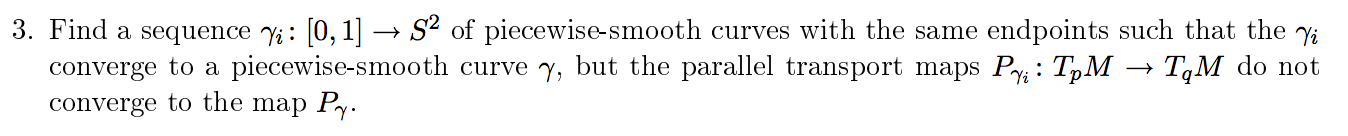
\includegraphics[width=0.7\textwidth]{geoII-s2-p3.png}
\end{figure}
\end{question}
\begin{solution} \hfill \\
All triangles in the discussion are great circle triangles.
From class, we saw that the parellel transport along a path of triangle, starting 
at a vertex and coming back to the chosen vertex, is given by a rotation of
$\theta - \pi$ where $\theta$ is the sum of three angles of the triangle, formed 
by the path. To discuss pointwise convergence, we choose the geodesic distance 
on $S^2$. Let $p$ be the north pole of $S^2$. Then, choose a triangle path, starting
at $p$ and coming back to $p$ such that $\theta - \pi > 0$. Now, for each $i \in 
\mathbb{N}$, choose a triangle path, $\gamma_{i}^{*}$, 
whose angle sum is $\theta'$, yet $\theta - \pi
= k \theta'$ for some $k \in \mathbb{N}$, and the path of the triangle is contained 
in $B(p,\dfrac{1}{i})$, and set $\gamma_i = (\gamma_i^*)^k$, which is the standard
path composition of $\gamma_i$ $k$ times.  Then, set $\gamma$
be the trivial path from $p$ to $p$ itself. Then, we see that $\gamma_i$ converges
to $\gamma$ pointwise, as for any $t \in [0,1]$, for any $\epsilon > 0$,
there exists $i$ such that $d(\gamma_i(t),\gamma(t)) < \epsilon$, whenever
$n \geq i$. Furthermore, $P_{\gamma_i}$ is given by a rotation of $\theta - \pi > 0$,
yet $P_{\gamma} = I$, so we see that $P_{\gamma_i}$ does not converge to $P_{\gamma}$
as a linear map. Hence, we have the desired construction. \hfill $\qed$ 
\end{solution}

\newpage

\begin{question}[1-4]
\hfill
\begin{figure}[h!]
  \centering
    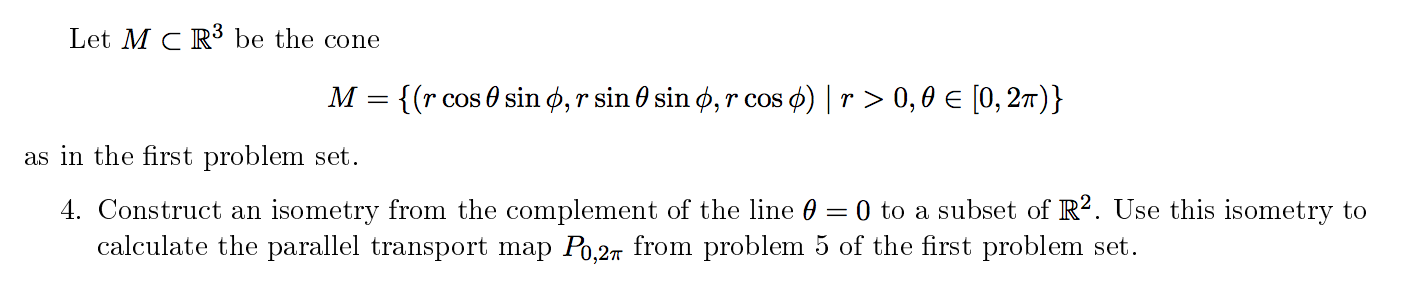
\includegraphics[width=0.7\textwidth]{geoII-s2-p4.png}
\end{figure}
\end{question}
\begin{solution} \hfill \\
Cutting the cone and unfolding it, and using elementary geometry tell us that,
in order to have an isometry, we must satisfy $r\sin(\phi)\theta = r\theta'$,
because the radius of the circle changes from $r\sin(\phi)$ to $r$, by unfolding.
As a parellel transport along any curve in $\mathbb{R}^2$ is an identity, we have 
that a parellel transport on the image is given by $(\cos(\theta'),-r\sin(\theta);
\sin(\theta'), -r\cos(\theta'))$. 
 
\end{solution}

\end{document}
